\section{Support Vector Machine (SVM)}
% Approach and results with respect to the SVM

\subsection{Radial Basis Function (RBF)}
% What is this kernel (broadly)

% Used Built-in implementation

% - Display graphs with hyper-param tuning (gradient based)
%   - How to for linear?
%   - possibly do analysis on embedded features to determine best features?

% - Mis-classifications analysis:
%   - check the original sentences (e.g. sentence length, good & bad words)
%   - which features common to tp, fp, tn, fn, any sentences that don't correlate

%  metrics: {'accuracy': 0.9753333333333334, 'f1_score': 0.9757377049180328, 'sensitivity': 0.9674902470741222, 'false_negative_rate': 0.032509752925877766, 'false_positive_rate': 0.016415868673050615, 'specificity': 0.9835841313269493}

The RBF kernel used was the built-in implementation provided within \verb|sklearn.svm.SVC|.\\
The hyper-parameters for the RBF kernel model where \verb|C|: the regularisation parameter (L2), \verb|gamma|: a coefficient used by the kernel.\\
The hyper-parameters were optimised through 5-fold cross-validation, within a grid search of C (within the range of 0.1 - 1, with 9 total steps) and gamma (within the range of 0.5 - 3, with 8 total steps).\\
The hyper-parameter tuning produced the following values: C = 0.97, Gamma = 2.2857142857142856.\\
The tuning has been visualised within \autoref{fig:rbf_hp}, with the optimal hyper-parameters shown by the red cross.
\begin{figure}[h!]
    \centering
    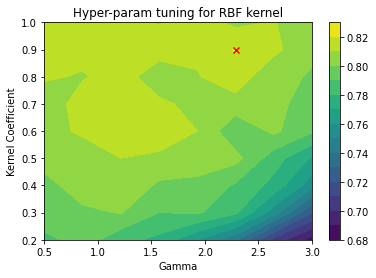
\includegraphics[width=0.6\textwidth]{figures/final/rbf.png}
    \caption{\label{fig:rbf_hp} Contour of RBF kernel model hyper-parameter tuning}
\end{figure}

Once the hyper-parameters were tuned, the model was then trained on the training set, and evaluated against the testing set.
This yielded the following metrics:\\
Accuracy: 0.9753333333333334, 
F1 Score: 0.9757377049180328, 
Sensitivity: 0.9674902470741222, 
False Negative rate: 0.032509752925877766, 
False Positive rate: 0.016415868673050615, 
Specificity: 0.9835841313269493.

The high accuracy indicates very little over-fitting.

\subsection{Polynomial}
% What is this kernel (broadly)

% Used Built-in implementation

% - Display graphs with hyper-param tuning (gradient based)
%   - How to for linear?
%   - possibly do analysis on embedded features to determine best features?

% - Mis-classifications analysis:
%   - check the original sentences (e.g. sentence length, good & bad words)
%   - which features common to tp, fp, tn, fn, any sentences that don't correlate

%  metrics: {'accuracy': 0.982, 'f1_score': 0.9822485207100592, 'sensitivity': 0.9713914174252276, 'false_negative_rate': 0.02860858257477243, 'false_positive_rate': 0.006839945280437756, 'specificity': 0.9931600547195623}
The Polynomial kernel used was also a built-in implementation provided within \verb|sklearn.svm.SVC|.\\
The hyper-parameters for the Polynomial kernel model where \verb|C|: the regularisation parameter (L2), \verb|gamma|: a coefficient used by the kernel, \verb|degree|: the maximum exponent for the polynomial used.\\
The hyper-parameters were optimised through 5-fold cross-validation, within a grid search of C (within the range of 0.1 - 1, with 9 total steps), gamma (within the range of 0.5 - 3, with 8 total steps), and degree (within the range of 1 - 3, with 3 total steps).\\
The hyper-parameter tuning produced the following values: C = 0.71, Gamma = 2.2857142857142856, Degree: 2.\\
Due to there being more than 2 parameters to tune, it isn't possible to visualise a contour for all dimensions. However you can perform a pair-wise contours, where you fix one parameter (using the optimal value) and plot the contour of the other parameters.\\ 
Contours can be found under \autoref{app:poly_hp}, in \autoref{fig:poly_hp_c_d}, \autoref{fig:poly_c_g}, and \autoref{fig:poly_g_d}.

Once the hyper-parameters were tuned, the model was then trained on the training set, and evaluated against the testing set.
This yielded the following metrics:\\
Accuracy: 0.982, 
F1 Score: 0.9822485207100592, 
Sensitivity: 0.9713914174252276, 
False Negative rate: 0.02860858257477243, 
False Positive rate: 0.006839945280437756, 
Specificity: 0.9931600547195623.

\subsection{Linear}
% What is this kernel (broadly)
% Top 3 positively correlated features:
% 300    0.282470
% 55     0.253391
% 5      0.225303
% Name: y, dtype: float64
% Top 3 negatively correlated features:
% 317   -0.285555
% 180   -0.248269
% 177   -0.247295
% Name: y, dtype: float64
% Used own implementation (what was the aim?)

% - Display graphs with hyper-param tuning (gradient based)
%   - How to for linear?
%   - possibly do analysis on embedded features to determine best features?

% - Mis-classifications analysis:
%   - check the original sentences (e.g. sentence length, good & bad words)
%   - which features common to tp, fp, tn, fn, any sentences that don't correlate

% Correct Predicitons: TP: 663, TN: 637
% Incorrect Predictions: FP: 94, FN: 106
%  metrics: {'accuracy': 0.8666666666666667, 'f1_score': 0.8689384010484927, 'sensitivity': 0.8621586475942783, 'false_negative_rate': 0.1378413524057217, 'false_positive_rate': 0.12859097127222982, 'specificity': 0.8714090287277702}

The Linear kernel used was created by ourselves. It should work by applying a weight to 6 specific features identified from the embedding that are most correlated (3 positively, 3 negatively) to the review sentiment.\\
The features were: 300 (correlation: 0.282470), 55 (0.253391), 5 (0.225303), 317 (-0.285555), 180 (-0.248269), and 177 (-0.247295)\\

The hyper-parameters for the Linear kernel model where \verb|C|: the regularisation parameter (L2), and 6 weights for each feature.\\
The hyper-parameters were optimised through 5-fold cross-validation, within a grid search of C (within the range of 0.1 - 1, with 9 total steps) and each of the 6 weights (within the range of 1 - 5, with 3 total steps for each feature).\\
The hyper-parameter tuning produced the following values: C = 0.7, weight for 300 = 3, weight for 55 = 3, weight for 5 = 1, weight for 317 = 3, weight for 180 = 5, and weight for 177 = 1.\\
As with the polynomial kernel model, a contour for all features isn't possible, however you can find contours for each weight paired with C under \autoref{app:lin_hp} in \autoref{fig:lin_300}, \autoref{fig:lin_55}, \autoref{fig:lin_5}, \autoref{fig:lin_317}, \autoref{fig:lin_180}, and \autoref{fig:lin_177}.

Once the hyper-parameters were tuned, the model was then trained on the training set, and evaluated against the testing set.
This yielded the following metrics:\\
Accuracy: 0.8666666666666667, 
F1 Score: 0.8689384010484927, 
Sensitivity: 0.8621586475942783, 
False Negative rate: 0.1378413524057217, 
False Positive rate: 0.12859097127222982, 
Specificity: 0.8714090287277702.

The above metrics show that this kernel is both over-fitting and under-fitting, with a greater than 10\% False Positive and Negative Rate.

\subsection{Kernel Comparison}
Under \autoref{app:svm_evaluation} you can find the confusion matrices for each model.\\
Along with the metrics above, and the confusion matrices, you can the RBF and Polynomial kernels significantly outperforming the Linear kernel.\\
This could possibly be due to the linear kernel being impacted by sentence length. The tables shown in \autoref{tab:lin_wc}, \autoref{tab:poly_wc}, and \autoref{tab:rbf_wc} show the RBF and Polynomial kernels more often correctly classifying shorter sentences. However the Linear kernel doesn't seem to have any correlation between sentence length and classification accuracy.

